\chapter{Using Subqueries to Solve Queries}

\section{\textbf{Practice 7}}

%--------------------------------------
\subsubsection*{Problem 01}
\addcontentsline{toc}{subsection}{Problem 01}
The HR department needs a query that prompts the user for an employee last name. The query then displays the last name and hire date of any employee in the same department as the employee whose name they supply (excluding that employee). For example, if the user enters Zlotkey, find all employees who work with Zlotkey (excluding Zlotkey).

\begin{frame}

\AddToShipoutPictureFG*{ % Add figure to foreground of current page
  \put(\LenToUnit{5.5cm},\LenToUnit{3cm}){% Adjust the coordinates as needed
    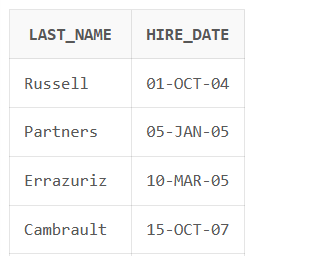
\includegraphics[width=7cm]{Figs/fig_701.png}
  }
}

\lstset{
  basicstyle=\fontsize{10}{12}\selectfont\ttfamily
}

\begin{lstlisting}[language=SQL]
SSELECT 	last_name,
       	TO_CHAR (hire_date, 'DD-MON-YY') hire_date
FROM 	hr.employees
WHERE 	department_id = (
         	SELECT 	department_id
         	FROM 	hr.employees
         	WHERE 	last_name = 'Zlotkey'
   		)
      	AND last_name <> initcap ('Zlotkey');
\end{lstlisting}
\textbf{Output: }
\end{frame}


%--------------------------------------
\newpage
\subsubsection*{Problem 02}
\addcontentsline{toc}{subsection}{Problem 02}
Create a report that displays the employee number, last name, and salary of all employees who earn more than the average salary. Sort the results in order of ascending salary.

\begin{frame}

\AddToShipoutPictureFG*{ % Add figure to foreground of current page
  \put(\LenToUnit{5.5cm},\LenToUnit{13cm}){% Adjust the coordinates as needed
    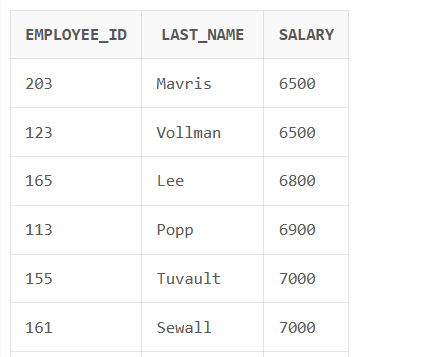
\includegraphics[width=7cm]{Figs/fig_702.png}
  }
}

\lstset{
  basicstyle=\fontsize{10}{12}\selectfont\ttfamily
}

\begin{lstlisting}[language=SQL]
SELECT 	employee_id, last_name, salary
FROM 	hr.employees
WHERE 	salary > (
   			SELECT AVG (salary)
   			FROM 	hr.employees
		)
ORDER BY salary;
\end{lstlisting}
\textbf{Output: }
\end{frame}




%--------------------------------------
\vspace{5cm}
\subsubsection*{Problem 03}
\addcontentsline{toc}{subsection}{Problem 03}
Write a query that displays the employee number and last name of all employees who work in a department with any employee whose last name contains the letter u. Save your SQL statement as lab\_07\_03.sql. Run your query.

\begin{frame}

\AddToShipoutPictureFG*{ % Add figure to foreground of current page
  \put(\LenToUnit{13cm},\LenToUnit{2.3cm}){% Adjust the coordinates as needed
    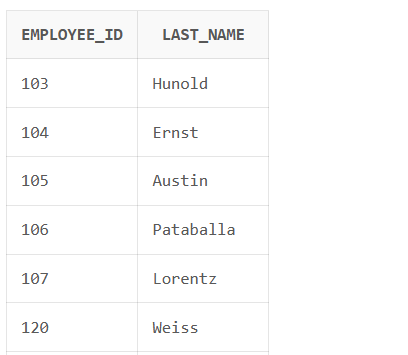
\includegraphics[width=7cm]{Figs/fig_703.png}
  }
}

\lstset{
  basicstyle=\fontsize{10}{12}\selectfont\ttfamily
}

\begin{lstlisting}[language=SQL]
SELECT 	employee_id,
       	last_name
FROM 	hr.employees
WHERE 	department_id IN (
   			SELECT department_id
   			FROM hr.employees
   			WHERE last_name LIKE '%u%'
		);
\end{lstlisting}
\textbf{Output: }
\end{frame}


%--------------------------------------
\newpage
\subsubsection*{Problem 04}
\addcontentsline{toc}{subsection}{Problem 04}
The HR department needs a report that displays the last name, department number, and job ID of all employees whose department location ID is 1700.

\begin{frame}

\AddToShipoutPictureFG*{ % Add figure to foreground of current page
  \put(\LenToUnit{13cm},\LenToUnit{14cm}){% Adjust the coordinates as needed
    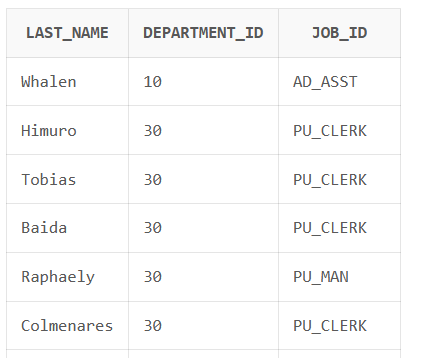
\includegraphics[width=7cm]{Figs/fig_704.png}
  }
}

\lstset{
  basicstyle=\fontsize{10}{12}\selectfont\ttfamily
}

\begin{lstlisting}[language=SQL]
SELECT 	last_name, department_id, job_id
FROM 	hr.employees
WHERE 	department_id IN (
   			SELECT 	department_id
   			FROM 	hr.departments
   			WHERE 	location_id = 1700
		)
ORDER BY department_id;
\end{lstlisting}
\textbf{Output: }
\end{frame}

%--------------------------------------
\vspace{5cm}
Modify the query so that the user is prompted for a location ID. Save this to a file named lab\_07\_04.sql.

\begin{frame}

\AddToShipoutPictureFG*{ % Add figure to foreground of current page
  \put(\LenToUnit{5.5cm},\LenToUnit{4cm}){% Adjust the coordinates as needed
    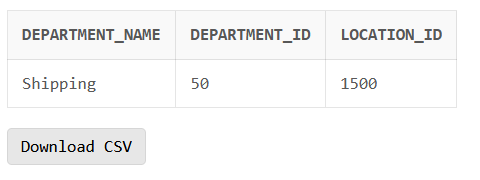
\includegraphics[width=7cm]{Figs/fig_704b.png}
  }
}

\lstset{
  basicstyle=\fontsize{10}{12}\selectfont\ttfamily
}

\begin{lstlisting}[language=SQL]
SELECT 	department_name, department_id, location_id
FROM 	hr.departments
WHERE 	location_id IN (
   			SELECT 	location_id
   			FROM 	hr.locations
   			WHERE 	location_id = 1500
		)
ORDER BY location_id;
\end{lstlisting}
\textbf{Output: }
\end{frame}



%--------------------------------------
\newpage
\subsubsection*{Problem 05}
\addcontentsline{toc}{subsection}{Problem 05}
Create a report for HR that displays the last name and salary of every employee who reports to King.
\begin{frame}

\AddToShipoutPictureFG*{ % Add figure to foreground of current page
  \put(\LenToUnit{5.5cm},\LenToUnit{14cm}){% Adjust the coordinates as needed
    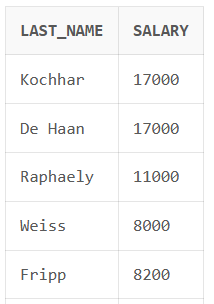
\includegraphics[width=4cm]{Figs/fig_705.png}
  }
}

\lstset{
  basicstyle=\fontsize{10}{12}\selectfont\ttfamily
}

\begin{lstlisting}[language=SQL]
SELECT 	last_name, salary
FROM 	hr.employees
WHERE 	manager_id IN (
   			SELECT 	employee_id
   			FROM 	hr.employees
   			WHERE 	last_name = 'King'
		);
\end{lstlisting}
\textbf{Output: }
\end{frame}



%--------------------------------------
\vspace{5cm}
\subsubsection*{Problem 06}
\addcontentsline{toc}{subsection}{Problem 06}
Create a report for HR that displays the department number, last name, and job ID for every employee in the Executive department.

\begin{frame}

\AddToShipoutPictureFG*{ % Add figure to foreground of current page
  \put(\LenToUnit{5.5cm},\LenToUnit{2.3cm}){% Adjust the coordinates as needed
    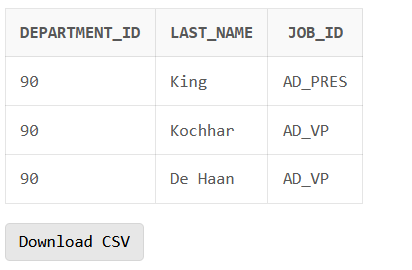
\includegraphics[width=7cm]{Figs/fig_706.png}
  }
}

\lstset{
  basicstyle=\fontsize{10}{12}\selectfont\ttfamily
}

\begin{lstlisting}[language=SQL]
SELECT 	department_id, last_name, job_id
FROM 	hr.employees
WHERE 	department_id = (
   			SELECT 	department_id
   			FROM 	hr.departments
   			WHERE 	department_name = 'Executive'
		);
\end{lstlisting}
\textbf{Output: }
\end{frame}


%--------------------------------------
\newpage
\subsubsection*{Problem 07}
\addcontentsline{toc}{subsection}{Problem 07}
Modify the query in lab\_07\_03.sql to display the employee number, last name, and salary of all employees who earn more than the average salary, and who work in a department with any employee whose last name contains a 'u'. Resave lab\_07\_03.sql as lab\_07\_07.sql. Run the statement in lab\_07\_03.sql.
\begin{frame}

\AddToShipoutPictureFG*{ % Add figure to foreground of current page
  \put(\LenToUnit{5.5cm},\LenToUnit{9cm}){% Adjust the coordinates as needed
    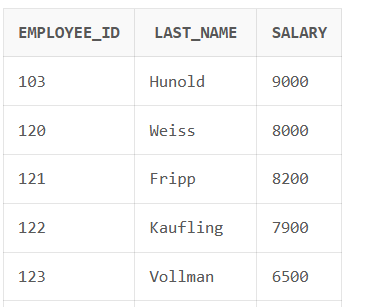
\includegraphics[width=8cm]{Figs/fig_707.png}
  }
}

\lstset{
  basicstyle=\fontsize{10}{12}\selectfont\ttfamily
}

\begin{lstlisting}[language=SQL]
SELECT 	employee_id, last_name, salary
FROM 	hr.employees
WHERE 	salary > (
         	SELECT AVG (salary)
         	FROM 	hr.employees
   		)
    AND department_id IN (
   			SELECT 	department_id
   			FROM 	hr.employees
   			WHERE last_name LIKE '%u%'
	);
\end{lstlisting}
\textbf{Output: }
\end{frame}


